% Options for packages loaded elsewhere
\PassOptionsToPackage{unicode}{hyperref}
\PassOptionsToPackage{hyphens}{url}
\PassOptionsToPackage{dvipsnames,svgnames,x11names}{xcolor}
%
\documentclass[
  letterpaper,
  DIV=11,
  numbers=noendperiod]{scrartcl}

\usepackage{amsmath,amssymb}
\usepackage{iftex}
\ifPDFTeX
  \usepackage[T1]{fontenc}
  \usepackage[utf8]{inputenc}
  \usepackage{textcomp} % provide euro and other symbols
\else % if luatex or xetex
  \usepackage{unicode-math}
  \defaultfontfeatures{Scale=MatchLowercase}
  \defaultfontfeatures[\rmfamily]{Ligatures=TeX,Scale=1}
\fi
\usepackage{lmodern}
\ifPDFTeX\else  
    % xetex/luatex font selection
\fi
% Use upquote if available, for straight quotes in verbatim environments
\IfFileExists{upquote.sty}{\usepackage{upquote}}{}
\IfFileExists{microtype.sty}{% use microtype if available
  \usepackage[]{microtype}
  \UseMicrotypeSet[protrusion]{basicmath} % disable protrusion for tt fonts
}{}
\makeatletter
\@ifundefined{KOMAClassName}{% if non-KOMA class
  \IfFileExists{parskip.sty}{%
    \usepackage{parskip}
  }{% else
    \setlength{\parindent}{0pt}
    \setlength{\parskip}{6pt plus 2pt minus 1pt}}
}{% if KOMA class
  \KOMAoptions{parskip=half}}
\makeatother
\usepackage{xcolor}
\setlength{\emergencystretch}{3em} % prevent overfull lines
\setcounter{secnumdepth}{-\maxdimen} % remove section numbering
% Make \paragraph and \subparagraph free-standing
\makeatletter
\ifx\paragraph\undefined\else
  \let\oldparagraph\paragraph
  \renewcommand{\paragraph}{
    \@ifstar
      \xxxParagraphStar
      \xxxParagraphNoStar
  }
  \newcommand{\xxxParagraphStar}[1]{\oldparagraph*{#1}\mbox{}}
  \newcommand{\xxxParagraphNoStar}[1]{\oldparagraph{#1}\mbox{}}
\fi
\ifx\subparagraph\undefined\else
  \let\oldsubparagraph\subparagraph
  \renewcommand{\subparagraph}{
    \@ifstar
      \xxxSubParagraphStar
      \xxxSubParagraphNoStar
  }
  \newcommand{\xxxSubParagraphStar}[1]{\oldsubparagraph*{#1}\mbox{}}
  \newcommand{\xxxSubParagraphNoStar}[1]{\oldsubparagraph{#1}\mbox{}}
\fi
\makeatother


\providecommand{\tightlist}{%
  \setlength{\itemsep}{0pt}\setlength{\parskip}{0pt}}\usepackage{longtable,booktabs,array}
\usepackage{calc} % for calculating minipage widths
% Correct order of tables after \paragraph or \subparagraph
\usepackage{etoolbox}
\makeatletter
\patchcmd\longtable{\par}{\if@noskipsec\mbox{}\fi\par}{}{}
\makeatother
% Allow footnotes in longtable head/foot
\IfFileExists{footnotehyper.sty}{\usepackage{footnotehyper}}{\usepackage{footnote}}
\makesavenoteenv{longtable}
\usepackage{graphicx}
\makeatletter
\def\maxwidth{\ifdim\Gin@nat@width>\linewidth\linewidth\else\Gin@nat@width\fi}
\def\maxheight{\ifdim\Gin@nat@height>\textheight\textheight\else\Gin@nat@height\fi}
\makeatother
% Scale images if necessary, so that they will not overflow the page
% margins by default, and it is still possible to overwrite the defaults
% using explicit options in \includegraphics[width, height, ...]{}
\setkeys{Gin}{width=\maxwidth,height=\maxheight,keepaspectratio}
% Set default figure placement to htbp
\makeatletter
\def\fps@figure{htbp}
\makeatother
% definitions for citeproc citations
\NewDocumentCommand\citeproctext{}{}
\NewDocumentCommand\citeproc{mm}{%
  \begingroup\def\citeproctext{#2}\cite{#1}\endgroup}
\makeatletter
 % allow citations to break across lines
 \let\@cite@ofmt\@firstofone
 % avoid brackets around text for \cite:
 \def\@biblabel#1{}
 \def\@cite#1#2{{#1\if@tempswa , #2\fi}}
\makeatother
\newlength{\cslhangindent}
\setlength{\cslhangindent}{1.5em}
\newlength{\csllabelwidth}
\setlength{\csllabelwidth}{3em}
\newenvironment{CSLReferences}[2] % #1 hanging-indent, #2 entry-spacing
 {\begin{list}{}{%
  \setlength{\itemindent}{0pt}
  \setlength{\leftmargin}{0pt}
  \setlength{\parsep}{0pt}
  % turn on hanging indent if param 1 is 1
  \ifodd #1
   \setlength{\leftmargin}{\cslhangindent}
   \setlength{\itemindent}{-1\cslhangindent}
  \fi
  % set entry spacing
  \setlength{\itemsep}{#2\baselineskip}}}
 {\end{list}}
\usepackage{calc}
\newcommand{\CSLBlock}[1]{\hfill\break\parbox[t]{\linewidth}{\strut\ignorespaces#1\strut}}
\newcommand{\CSLLeftMargin}[1]{\parbox[t]{\csllabelwidth}{\strut#1\strut}}
\newcommand{\CSLRightInline}[1]{\parbox[t]{\linewidth - \csllabelwidth}{\strut#1\strut}}
\newcommand{\CSLIndent}[1]{\hspace{\cslhangindent}#1}

\KOMAoption{captions}{tableheading}
\makeatletter
\@ifpackageloaded{caption}{}{\usepackage{caption}}
\AtBeginDocument{%
\ifdefined\contentsname
  \renewcommand*\contentsname{Table of contents}
\else
  \newcommand\contentsname{Table of contents}
\fi
\ifdefined\listfigurename
  \renewcommand*\listfigurename{List of Figures}
\else
  \newcommand\listfigurename{List of Figures}
\fi
\ifdefined\listtablename
  \renewcommand*\listtablename{List of Tables}
\else
  \newcommand\listtablename{List of Tables}
\fi
\ifdefined\figurename
  \renewcommand*\figurename{Figure}
\else
  \newcommand\figurename{Figure}
\fi
\ifdefined\tablename
  \renewcommand*\tablename{Table}
\else
  \newcommand\tablename{Table}
\fi
}
\@ifpackageloaded{float}{}{\usepackage{float}}
\floatstyle{ruled}
\@ifundefined{c@chapter}{\newfloat{codelisting}{h}{lop}}{\newfloat{codelisting}{h}{lop}[chapter]}
\floatname{codelisting}{Listing}
\newcommand*\listoflistings{\listof{codelisting}{List of Listings}}
\makeatother
\makeatletter
\makeatother
\makeatletter
\@ifpackageloaded{caption}{}{\usepackage{caption}}
\@ifpackageloaded{subcaption}{}{\usepackage{subcaption}}
\makeatother

\ifLuaTeX
  \usepackage{selnolig}  % disable illegal ligatures
\fi
\usepackage{bookmark}

\IfFileExists{xurl.sty}{\usepackage{xurl}}{} % add URL line breaks if available
\urlstyle{same} % disable monospaced font for URLs
\hypersetup{
  pdftitle={Advancing Renewable Energy in Buildings},
  pdfauthor={Juracy Américo de Oliveira Filho},
  colorlinks=true,
  linkcolor={blue},
  filecolor={Maroon},
  citecolor={Blue},
  urlcolor={Blue},
  pdfcreator={LaTeX via pandoc}}


\title{Advancing Renewable Energy in Buildings}
\usepackage{etoolbox}
\makeatletter
\providecommand{\subtitle}[1]{% add subtitle to \maketitle
  \apptocmd{\@title}{\par {\large #1 \par}}{}{}
}
\makeatother
\subtitle{Overcoming Challenges Through Policy and Innovation}
\author{Juracy Américo de Oliveira Filho}
\date{2024-09-04}

\begin{document}
\maketitle


\section{Agenda}\label{agenda}

\begin{enumerate}
\def\labelenumi{\arabic{enumi})}
\tightlist
\item
  Introduction\\
\item
  Agenda
\item
  Overview of the Energy Landscape
\item
  Challenges in the Building Sector
\item
  Potential Solutions: Policy and Innovation
\item
  Evaluation and Conclusion
\end{enumerate}

\textbf{To begin}, let's take a look at the agenda for today's
presentation. \textbf{First}, I will be giving a brief overview of the
current energy landscape and the challenges we face in the building
sector. \textbf{Then}, we'll move into a discussion of the major
roadblocks hindering the widespread adoption of renewable energy
technologies in our buildings. \textbf{Having established this
foundation}, I'll be outlining some potential solutions, focusing on the
crucial role of policy and innovation. \textbf{Finally}, I will evaluate
these solutions and offer some concluding thoughts.

\begin{itemize}
\tightlist
\item
\end{itemize}

\section{Energy Landscape}\label{energy-landscape}

\begin{itemize}
\tightlist
\item
  Growing Global Energy Demand
\item
  Climate Change and Energy Consumption
\item
  Building Sector's Impact:

  \begin{itemize}
  \tightlist
  \item
    Significant energy consumption
  \item
    High greenhouse gas emissions
  \end{itemize}
\item
  Importance of Renewable Energy
\end{itemize}

\emph{Note} Solar Classes - (\emph{Through the {Looking Glass}}, 2024)
Copyright ©~2024

\textbf{Let's start by considering the bigger picture}. As we all know,
the global demand for energy is constantly growing. Couple this with the
urgent need to address climate change and it becomes clear that we need
to rethink our approach to energy consumption, especially in the
building sector.

\textbf{Why the building sector, you might ask?} The reason is that
buildings account for a substantial portion of global energy consumption
and greenhouse gas emissions. This is where renewable energy sources
come in, offering a viable pathway to reduce the carbon footprint of
buildings and create a more sustainable future.

\begin{itemize}
\tightlist
\item
\end{itemize}

\section{Challenges in Renewable Energy
Adoption}\label{challenges-in-renewable-energy-adoption}

\begin{itemize}
\tightlist
\item
  High Upfront Costs
\item
  Technological Limitation
\item
  Lack of Public Awareness
\item
  Policy and Regulatory Inconsistencies
\end{itemize}

\begin{figure}

\centering{

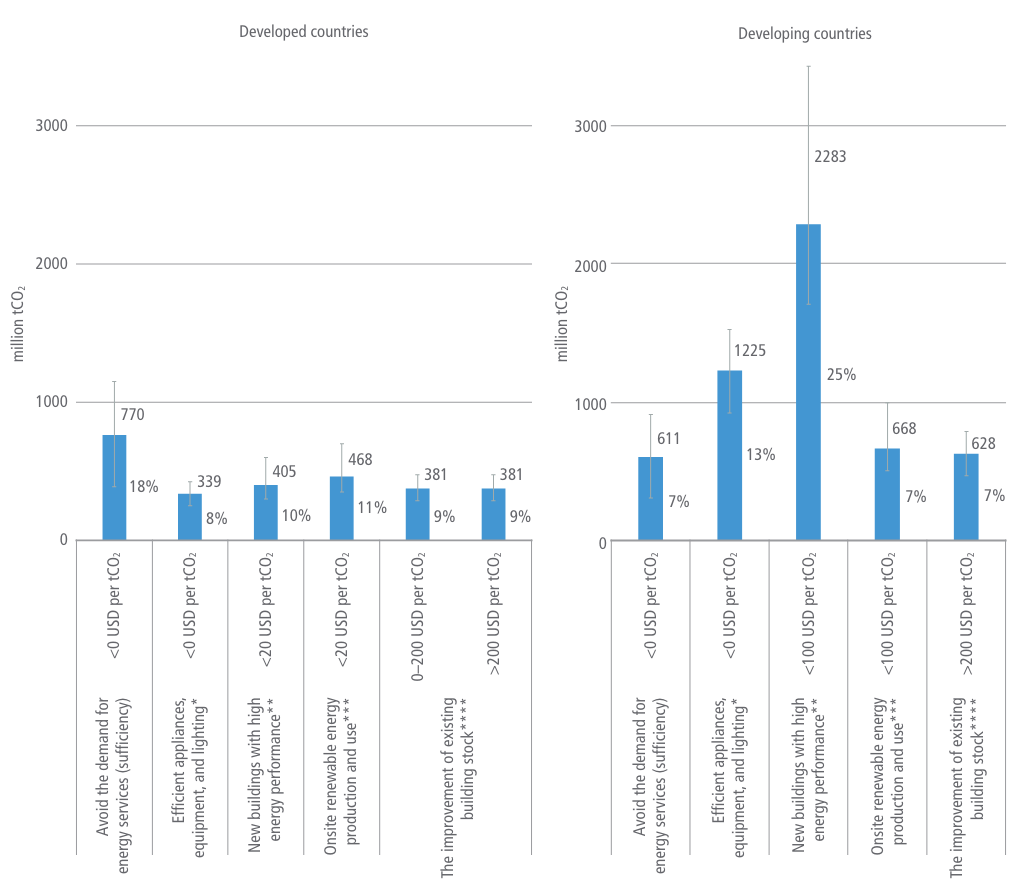
\includegraphics{Pastedimage20240901072851.png}

}

\caption{\label{fig-problens}GHG Emission}

\end{figure}%

\emph{Note.} Energy consumption trends over the past decade in developed
and developing countries. (Environment Program, 2020)

\textbf{Now, let's shift our attention to the heart of the matter: the
challenges we need to overcome.} Despite the promise of renewable
energy, its widespread adoption in buildings faces several obstacles.
\textbf{These barriers include}:

\begin{itemize}
\tightlist
\item
  \textbf{High upfront costs:} The initial investment required for
  renewable energy systems can be a deterrent for many building owners.
\item
  \textbf{Technological limitations}: While promising, some technologies
  are still under development and may not yet be efficient or
  cost-effective for all types of buildings.
\item
  \textbf{Lack of public awareness:} Many people are simply not aware of
  the benefits of renewable energy or the options available to them.
\item
  \textbf{Policy and regulatory inconsistencies}: A lack of clear,
  consistent policies and regulations can create uncertainty for
  investors and hinder the growth of the renewable energy market in the
  building sector.
\end{itemize}

\textbf{With these challenges in mind, let's explore some potential
solutions.}

\begin{itemize}
\tightlist
\item
\end{itemize}

\section{Solutions -- Policy
Approaches}\label{solutions-policy-approaches}

\begin{itemize}
\tightlist
\item
  Role of Government Policy

  \begin{itemize}
  \tightlist
  \item
    Supportive policies needed
  \end{itemize}
\item
  Key Policy Measures

  \begin{itemize}
  \tightlist
  \item
    Building energy codes
  \item
    Financial incentives (tax credits, grants, subsidies)
  \item
    Capacity development and training programs
  \end{itemize}
\end{itemize}

\begin{figure}

\centering{

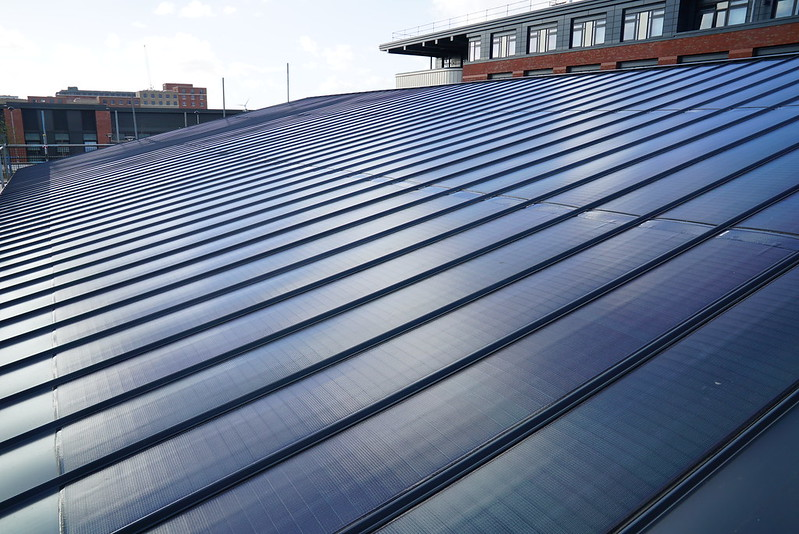
\includegraphics{Photovoltaic roof.jpg}

}

\caption{\label{fig-solutions}Photovoltaic Roof}

\end{figure}%

\emph{Note}. The building integrated a photovoltaic roof. (IKC, 2016).

\textbf{First}, let's talk about the role of government policy.

\begin{itemize}
\tightlist
\item
  Governments can play a significant role in promoting renewable energy
  use in buildings by implementing supportive policies.
\item
  This could include:

  \begin{itemize}
  \item
    Mandatory building energy codes that set minimum standards for
    energy efficiency and encourage renewable energy integration.
  \item
    Financial incentives such as tax credits, grants, and subsidies to
    make renewable energy systems more financially attractive.
  \item
    Programs to support capacity development and training for industry
    professionals on the design, installation, and maintenance of
    renewable energy systems.
  \end{itemize}
\end{itemize}

\begin{itemize}
\tightlist
\item
\end{itemize}

\section{Solutions -- Effective Policy
Instruments}\label{solutions-effective-policy-instruments}

\begin{itemize}
\tightlist
\item
  Renewable Portfolio Standards (RPS)
\item
  Renewable Energy Standards (RES)
\item
  Feed-in Tariffs
\end{itemize}

\begin{figure}

\centering{

\includegraphics{Green Buildings.webp}

}

\caption{\label{fig-solutions}Green Buildings}

\end{figure}%

\emph{Note}. Green Building Policy. (Team, 2023).

\textbf{In addition to these measures, several specific policy
instruments have proven effective in promoting renewable energy
adoption}.

\begin{itemize}
\tightlist
\item
  \textbf{Renewable Portfolio Standards (RPS)}: These policies require
  utilities to generate a certain percentage of their electricity from
  renewable sources.
\item
  \textbf{Renewable Energy Standards (RES)}: Similar to RPS, RES
  policies mandate a certain percentage of energy consumption to come
  from renewables.
\item
  \textbf{Feed-in tariffs:} These policies offer long-term contracts to
  renewable energy producers, guaranteeing a fixed price for the
  electricity they feed into the grid.
\end{itemize}

\begin{itemize}
\tightlist
\item
\end{itemize}

\section{Solutions -- Technological
Innovation}\label{solutions-technological-innovation}

\begin{itemize}
\tightlist
\item
  Need for Technological Advancements

  \begin{itemize}
  \tightlist
  \item
    Efficiency, affordability, accessibility
  \end{itemize}
\item
  Innovative Technologies:

  \begin{itemize}
  \tightlist
  \item
    Building-Integrated Photovoltaics (BIPV)
  \item
    Solar Thermal Technologies
  \item
    Geothermal Energy
  \item
    Micro-Wind Turbines
  \end{itemize}
\end{itemize}

\begin{figure}

\centering{


\includegraphics{GlassSolarPanel.jpg}

}

\caption{\label{fig-solutions}Solar Panel Architecture}

\end{figure}%

\emph{Note}. Seamlessly integrates photovoltaic technology into building
elements, turning them into efficient energy sources while offering
durability, sustainability, and financial incentives.. (\emph{Through
the {Looking Glass}}, 2024).

\textbf{Moving on to our second key area, innovation}, technological
advancements are essential to improve the efficiency, affordability, and
accessibility of renewable energy systems.

\begin{itemize}
\tightlist
\item
  Continued research and development of innovative renewable energy
  technologies are crucial for wider adoption in the building sector.
\item
  This includes:

  \begin{itemize}
  \tightlist
  \item
    Further development of building-integrated photovoltaics (BIPV) that
    seamlessly incorporate solar panels into building designs.
  \item
    Advancements in solar thermal technologies that use sunlight to heat
    water and air for buildings.
  \item
    Exploration of geothermal energy, utilizing the earth's heat for
    heating and cooling purposes.
  \item
    Development of micro-wind turbines that can generate electricity
    from wind in urban environments.
  \end{itemize}
\end{itemize}

\begin{itemize}
\tightlist
\item
\end{itemize}

\section{Importance of Energy
Storage}\label{importance-of-energy-storage}

\begin{itemize}
\tightlist
\item
  Addressing Intermittency

  \begin{itemize}
  \tightlist
  \item
    Ensuring reliable energy supply
  \end{itemize}
\item
  Key to consistent energy availability

  \begin{itemize}
  \tightlist
  \item
    Key to consistent energy availability
  \end{itemize}
\end{itemize}

\begin{figure}

\centering{

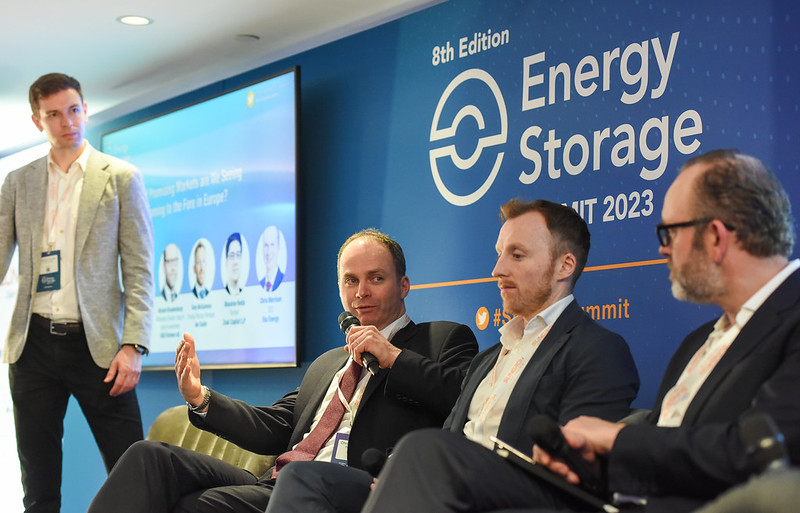
\includegraphics{Energy Storage.jpg}

}

\caption{\label{fig-solutions}Energy Storage}

\end{figure}%

\emph{Note}. Energy Storage Summit 2023 - Leonardo Royal Hotel, London,
United Kingdom. (Stanley-Tate, 2023).

\textbf{Another area where innovation is key is in energy storage}.
Improved energy storage solutions can address one of the main challenges
with renewable energy: its intermittency. By storing excess energy
generated during periods of high production, we can ensure a consistent
and reliable energy supply even when the sun isn't shining or the wind
isn't blowing.

\begin{itemize}
\tightlist
\item
\end{itemize}

\section{Evaluation of Solutions}\label{evaluation-of-solutions}

\begin{itemize}
\tightlist
\item
  Policy-Driven Approaches:

  \begin{itemize}
  \tightlist
  \item
    Effective in incentivizing adoption
  \item
    Challenges: inconsistencies, enforcement, priority shifts
  \end{itemize}
\item
  Technology-Driven Solutions:

  \begin{itemize}
  \tightlist
  \item
    Potential for increased efficiency and reduced costs
  \item
    Challenges: high costs, expertise required, risk of obsolescence
  \end{itemize}
\end{itemize}

\begin{figure}

\centering{

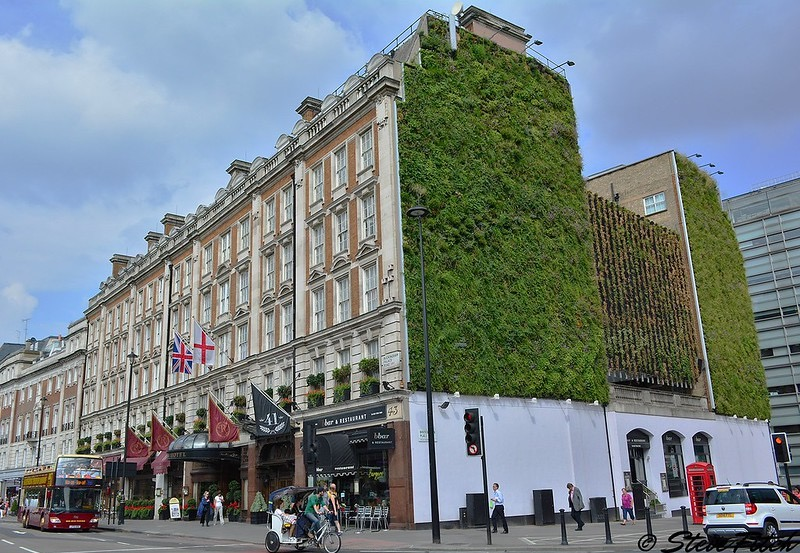
\includegraphics{LivingWall.jpg}

}

\caption{\label{fig-solutions}``Living wall''}

\end{figure}%

\emph{Note}. ``Living wall'' to enhance the building in London. (Steve
Fitch, 2014).

\textbf{Now that we've explored both policy and innovation, let's take a
moment to evaluate these solutions.}

\textbf{Policy-driven approaches can be highly effective}. By creating a
supportive policy environment, governments can incentivize the adoption
of renewable energy, attract investment, and drive market
transformation.

\begin{itemize}
\tightlist
\item
  \textbf{However}, there are also potential drawbacks.

  \begin{itemize}
  \tightlist
  \item
    Policy inconsistencies, lack of enforcement, and changes in
    government priorities can undermine the effectiveness of these
    measures.
  \end{itemize}
\end{itemize}

\textbf{Technology-driven solutions offer the promise of increased
efficiency, reduced costs over time, and the potential for breakthroughs
that can revolutionize the way we power our buildings}.

\begin{itemize}
\tightlist
\item
  \textbf{However,} these solutions are not without challenges.

  \begin{itemize}
  \tightlist
  \item
    High upfront costs, the need for specialized expertise, and the risk
    of technological obsolescence are factors that need to be carefully
    considered.
  \end{itemize}
\end{itemize}

\begin{itemize}
\tightlist
\item
\end{itemize}

\section{Conclusion}\label{conclusion}

\begin{itemize}
\tightlist
\item
  Balanced Approach Required:

  \begin{itemize}
  \tightlist
  \item
    Combination of policy and innovation
  \end{itemize}
\item
  Collaboration Needed:

  \begin{itemize}
  \tightlist
  \item
    Governments, industry leaders, individuals
  \end{itemize}
\item
  Focus on:

  \begin{itemize}
  \tightlist
  \item
    Encouraging investment and innovation
  \item
    Advancing technology for efficiency and affordability
  \end{itemize}
\item
  Goal:

  \begin{itemize}
  \tightlist
  \item
    Clean, sustainable energy for buildings
  \item
    Mitigating climate change, enhancing energy security
  \item
    Healthier planet for future generations
  \end{itemize}
\end{itemize}

\begin{figure}

\centering{

\includegraphics{sustainable architecture skills.webp}

}

\caption{\label{fig-solutions}Sustainable Architecture Skills}

\end{figure}%

\emph{Note}. Green building policies have become a global phenomenon.
(Team, 2023).

\textbf{In conclusion}, I believe that a balanced approach that combines
supportive policies with continuous technological innovation is the key
to unlocking the full potential of renewable energy in buildings.
Governments, industry leaders, and individuals must work together to
create a policy environment that encourages investment and innovation.
At the same time, continued technological advancements are needed to
make renewable energy systems more efficient, affordable, and
accessible. By embracing both policy and innovation, we can accelerate
the transition towards a future where our buildings are powered by
clean, sustainable energy, mitigating climate change, enhancing energy
security, and creating a healthier planet for generations to come. Thank
you.

\begin{itemize}
\tightlist
\item
\end{itemize}

\section{Slide Title}\label{slide-title}

L. Chen et al. (2024) Komurlu et al. (2024) Okwandu et al. (2024)
Environment Program (2020) Environment Program (2024) C. Chen et al.
(2022) Yang et al. (2023) Intergovernmental Panel on Climate Change
(IPCC) (2023) L. Chen et al. (2023) Babí Almenar et al. (2021)

\begin{itemize}
\tightlist
\item
\end{itemize}

\section{References}\label{references}

\phantomsection\label{refs}
\begin{CSLReferences}{1}{0}
\bibitem[\citeproctext]{ref-babialmenarNexusNaturebasedSolutions2021}
Babí Almenar, J., Elliot, T., Rugani, B., Philippe, B., Navarrete
Gutierrez, T., Sonnemann, G., \& Geneletti, D. (2021). Nexus between
nature-based solutions, ecosystem services and urban challenges.
\emph{Land Use Policy}, \emph{100}, 104898.
\url{https://doi.org/10.1016/j.landusepol.2020.104898}

\bibitem[\citeproctext]{ref-chenDynamicCharacteristicDecoupling2022}
Chen, C., Cao, X., Zhang, S., Lei, Z., \& Zhao, K. (2022). Dynamic
{Characteristic} and {Decoupling Relationship} of {Energy Consumption}
on {China}'s {Construction Industry}. \emph{Buildings}, \emph{12}(10,
10), 1745. \url{https://doi.org/10.3390/buildings12101745}

\bibitem[\citeproctext]{ref-chenArtificialIntelligencebasedSolutions2023}
Chen, L., Chen, Z., Zhang, Y., Liu, Y., Osman, A. I., Farghali, M., Hua,
J., Al-Fatesh, A., Ihara, I., Rooney, D. W., \& Yap, P.-S. (2023).
Artificial intelligence-based solutions for climate change: A review.
\emph{Environmental Chemistry Letters}, \emph{21}(5), 2525--2557.
\url{https://doi.org/10.1007/s10311-023-01617-y}

\bibitem[\citeproctext]{ref-chenGreenBuildingPractices2024}
Chen, L., Hu, Y., Wang, R., Li, X., Chen, Z., Hua, J., Osman, A. I.,
Farghali, M., Huang, L., Li, J., Dong, L., Rooney, D. W., \& Yap, P.-S.
(2024). Green building practices to integrate renewable energy in the
construction sector: A review. \emph{Environmental Chemistry Letters},
\emph{22}(2), 751--784. \url{https://doi.org/10.1007/s10311-023-01675-2}

\bibitem[\citeproctext]{ref-environmentprogramu.n.BuildingsEnergySystem2020}
Environment Program, U. N. (2020). \emph{Buildings - {Energy System}}.
IEA. \url{https://www.iea.org/energy-system/buildings}

\bibitem[\citeproctext]{ref-environmentprogramu.n.GlobalStatusReport2024}
Environment Program, U. N. (2024, March 6). \emph{Global {Status Report}
for {Buildings} and {Construction} \textbar{} {UNEP} - {UN Environment
Programme}}.
\url{https://www.unep.org/resources/report/global-status-report-buildings-and-construction}

\bibitem[\citeproctext]{ref-ikcBIPVcoIntegratedRoof2016}
IKC, S. (2016). \emph{{BIPVco Integrated Roof}} {[}Graphic{]}.
\url{https://www.flickr.com/photos/specific-ikc/30088006605/}

\bibitem[\citeproctext]{ref-intergovernmentalpanelonclimatechangeipccBuildings2023}
Intergovernmental Panel on Climate Change (IPCC) (Ed.). (2023).
Buildings. In \emph{Climate {Change} 2022 - {Mitigation} of {Climate
Change}: {Working Group III Contribution} to the {Sixth Assessment
Report} of the {Intergovernmental Panel} on {Climate Change}} (pp.
953--1048). Cambridge University Press.
\url{https://doi.org/10.1017/9781009157926.011}

\bibitem[\citeproctext]{ref-komurluExploringBarriersManaging2024}
Komurlu, R., Kalkan Ceceloglu, D., \& Arditi, D. (2024). Exploring the
{Barriers} to {Managing Green Building Construction Projects} and
{Proposed Solutions}. \emph{Sustainability}, \emph{16}(13, 13), 5374.
\url{https://doi.org/10.3390/su16135374}

\bibitem[\citeproctext]{ref-okwanduRolePolicyRegulation2024}
Okwandu, A. C., Esho, A. O.-O., Iluyomade, T. D., Olatunde, T. M.,
Okwandu, A. C., Esho, A. O.-O., Iluyomade, T. D., \& Olatunde, T. M.
(2024). The role of policy and regulation in promoting green buildings.
\emph{World Journal of Advanced Research and Reviews}, \emph{22}(1, 1),
139--150. \url{https://doi.org/10.30574/wjarr.2024.22.1.1047}

\bibitem[\citeproctext]{ref-stanley-tateEnergyStorageSummit2023}
Stanley-Tate, D. (2023). \emph{Energy {Storage Summit} 2023}
{[}Graphic{]}.
\url{https://www.flickr.com/photos/194605019@N03/52708970693/}

\bibitem[\citeproctext]{ref-stevefitchLivingWallEnhance2014}
Steve Fitch. (2014). \emph{"{Living} wall" to enhance the building.
{London}} {[}Graphic{]}.
\url{https://www.flickr.com/photos/111683772@N02/14529433557/}

\bibitem[\citeproctext]{ref-teamGreenBuildingPolicy2023}
Team, V. E. G. M. (2023, September 21). \emph{Green {Building Policy
Evolution}: 2023 \& {Beyond}}. Vert Energy Group.
\url{https://vertenergygroup.com/the-evolution-of-green-building-policy-in-2023-and-beyond/}

\bibitem[\citeproctext]{ref-LookingGlassRole2024}
\emph{Through the {Looking Glass}: {The Role} of {Solar Glass} in
{Advancing Solar Panel Architecture}}. (2024, May 31).
\url{https://www.mitrex.com/blog/through-the-looking-glass-the-role-of-solar-glass-in-advancing-solar-panel-architecture}

\bibitem[\citeproctext]{ref-yangCircularEconomyStrategies2023}
Yang, M., Chen, L., Wang, J., Msigwa, G., Osman, A. I., Fawzy, S.,
Rooney, D. W., \& Yap, P.-S. (2023). Circular economy strategies for
combating climate change and other environmental issues.
\emph{Environmental Chemistry Letters}, \emph{21}(1), 55--80.
\url{https://doi.org/10.1007/s10311-022-01499-6}

\end{CSLReferences}

\begin{itemize}
\tightlist
\item
\end{itemize}

\section{Q\&A}\label{qa}




\end{document}
